% Created 2025-02-28 Fri 14:25
\documentclass[10pt]{article}
\usepackage{graphicx}
\usepackage{longtable}
\usepackage{wrapfig}
\usepackage{rotating}
\usepackage[normalem]{ulem}
\usepackage{amsmath}
\usepackage{amssymb}
\usepackage{capt-of}
\usepackage{hyperref}
\usepackage[newfloat]{minted}
\usepackage[a4paper, total={6.5in, 9in}]{geometry}
\usepackage{minted}
\setminted{breaklines}
\usepackage[utf8]{inputenc}
\renewcommand{\familydefault}{\sfdefault}
\usemintedstyle{vs}
\usepackage[most]{tcolorbox}
\usepackage{CJKutf8}
\usepackage{xurl}
\usepackage{fontawesome5}
\usepackage{hyperref}
\usepackage{graphicx}
\usepackage{float}
\author{Vincent Conus\thanks{vincent.conus@protonmail.com}}
\date{2024-01-31}
\title{KRIA board Vitis IDE setup}
\hypersetup{
 pdfauthor={Vincent Conus},
 pdftitle={KRIA board Vitis IDE setup},
 pdfkeywords={},
 pdfsubject={A guide to setup Xilinx's Vitis IDE},
 pdfcreator={Emacs 29.4 (Org mode 9.6.15)}, 
 pdflang={English}}
\begin{document}

\maketitle
\tableofcontents

\section{Setting up the IDE}
\label{sec:orgdf9de98}
Xilinx's Vitis IDE is the recommended tool used to build software for the Xilinx boards.
It also include the tools to interact with the FPGA part, making the whole
software very large (around 200GB of disk usage).

However, this large tool-set allows for a convenient development environment, in particular
in our case where some FreeRTOS system, with many dependencies is to be build.

The installer can be found on Xilinx download page\footnote{\url{https://www.xilinx.com/support/download/index.html/content/xilinx/en/downloadNav/vitis.html}}. You will need to get
a file named something like \texttt{Xilinx\_Unified\_2022.2\_1014\_8888\_Lin64.bin}\footnote{The name of the installer binary file might change as a new version of
the IDE is release every year or so.}.

Vitis IDE installer is compatible with versions of Ubuntu, among other distributions,
but not officially yet for the 22.04 version.
Furthermore, the current install was tested on Pop OS, a distribution derived from Ubuntu.
However, even with this more unstable status, no major problems were encountered
with this tool during the development stages.

This guide will present a setup procedure that supposedly works for all distributions based on the newest
LTS from Ubuntu. For other Linux distributions or operating system, please refer to the official documentation.

\subsection{Dependencies \& installation}
\label{sec:orgb086230}
Some packages are required to be installed on the host system
in order for the installation process to happen successfully:

\begin{minted}[frame=single,framesep=2mm,baselinestretch=1.2,linenos,breaklines,fontsize=\footnotesize]{sh}
sudo apt-get -y update

sudo apt-get -y install libncurses-dev \
     ncurses-term \
     ncurses-base \
     ncurses-bin \
     libncurses5 \
     libtinfo5 \
     libncurses5-dev \
     libncursesw5-dev
\end{minted}

Once this is done, the previously downloaded binary installer can be executed:

\begin{minted}[frame=single,framesep=2mm,baselinestretch=1.2,linenos,breaklines,fontsize=\footnotesize]{sh}
./Xilinx_Unified_2022.2_1014_8888_Lin64.bin
\end{minted}

If it is not possible to run the previous command, make the file executable with the \texttt{chmod} command:

\begin{minted}[frame=single,framesep=2mm,baselinestretch=1.2,linenos,breaklines,fontsize=\footnotesize]{sh}
sudo chmod +x ./Xilinx_Unified_2022.2_1014_8888_Lin64.bin
\end{minted}

From there you can follow the step-by-step graphical installer.
The directory chosen for the rest of this guide for the Xilinx directory
is directly the \texttt{\$HOME}, but the installation can be set elsewhere is needed.

\begin{tcolorbox}[colback=orange!5!white,colframe=orange!75!black]
\textbf{WARNING}: This whole procedure can take up to multiple hours to complete
and is prone to failures (regarding missing dependencies, typically),
so your schedule should be arranged accordingly.
\end{tcolorbox}

\subsection{Platform configuration file}
\label{sec:orgeb0492f}
With a Xilinx account, a \texttt{.bsp} archive can be downloaded for the taget platform\footnote{\url{https://www.xilinx.com/member/forms/download/xef.html?filename=xilinx-kr260-starterkit-v2022.2-10141622.bsp}}.

Once the file is downloaded, the following commands allows to "un-tar" it,
making th needed \texttt{.xsa} file accessible via a file explorer.

\begin{minted}[frame=single,framesep=2mm,baselinestretch=1.2,linenos,breaklines,fontsize=\footnotesize]{sh}
tar xvfz xilinx-kr260-starterkit-v2022.2-10141622.bsp
ls xilinx-kr260-starterkit-2022.2/hardware/xilinx-kr260-starterkit-2022.2/
\end{minted}


\subsection{[DEPRECATED] Platform configuration file generation}
\label{sec:org72600a1}
In order to have the libraries and configurations in the IDE ready to be used for our board,
we need to obtain some configuration files that are specific for the Kria KV260,
as presented in the Xilinx guide for Kria and Vitis\footnote{\url{https://xilinx.github.io/kria-apps-docs/kv260/2022.1/build/html/docs/build\_vitis\_platform.html?highlight=xsa}}.

A Xilinx dedicated repository\footnote{\url{https://github.com/Xilinx/kria-vitis-platforms}} is available for us to download  such configurations,
but they required to be built.

As for the dependencies, \texttt{Cmake}, \texttt{tcl} and \texttt{idn} will become needed in order to build the firmware.
Regarding \texttt{idn}, some version issue can happen, but as discussed in a thread on Xilinx's forum\footnote{\url{https://support.xilinx.com/s/question/0D52E00006jrzsYSAQ/platform-project-cannot-be-created-on-vitis?language=en\_US}},
if \texttt{libidn11} is specifically required but not available (it is the case for Ubuntu 22.04),
creating a symbolic link from the current, 12 version works as a workaround.

Here are the steps for installing the dependencies and building this configuration file:

\begin{minted}[frame=single,framesep=2mm,baselinestretch=1.2,linenos,breaklines,fontsize=\footnotesize]{sh}
sudo apt-get update
sudo apt-get install cmake tcl libidn11-dev \
     libidn-dev libidn12 idn
sudo ln -s /usr/lib/x86_64-linux-gnu/libidn.so.12 \
     /usr/lib/x86_64-linux-gnu/libidn.so.11

cd ~/Xilinx
git clone --recursive \
    https://github.com/Xilinx/kria-vitis-platforms.git
cd kria-vitis-platforms/k26/platforms
export XILINX_VIVADO=/home/$USER/Xilinx/Vivado/2022.2/
export XILINX_VITIS=/home/$USER/Xilinx/Vitis/2022.2/
make platform PLATFORM=k26_base_starter_kit
\end{minted}

\section{Setting up and building a new project for the Kria board}
\label{sec:org8359973}
With the platform configuration files available, we can now use the IDE to generate a
new project for our board. The whole process will be described with screen captures and
captions.

\begin{figure}[htbp]
\centering
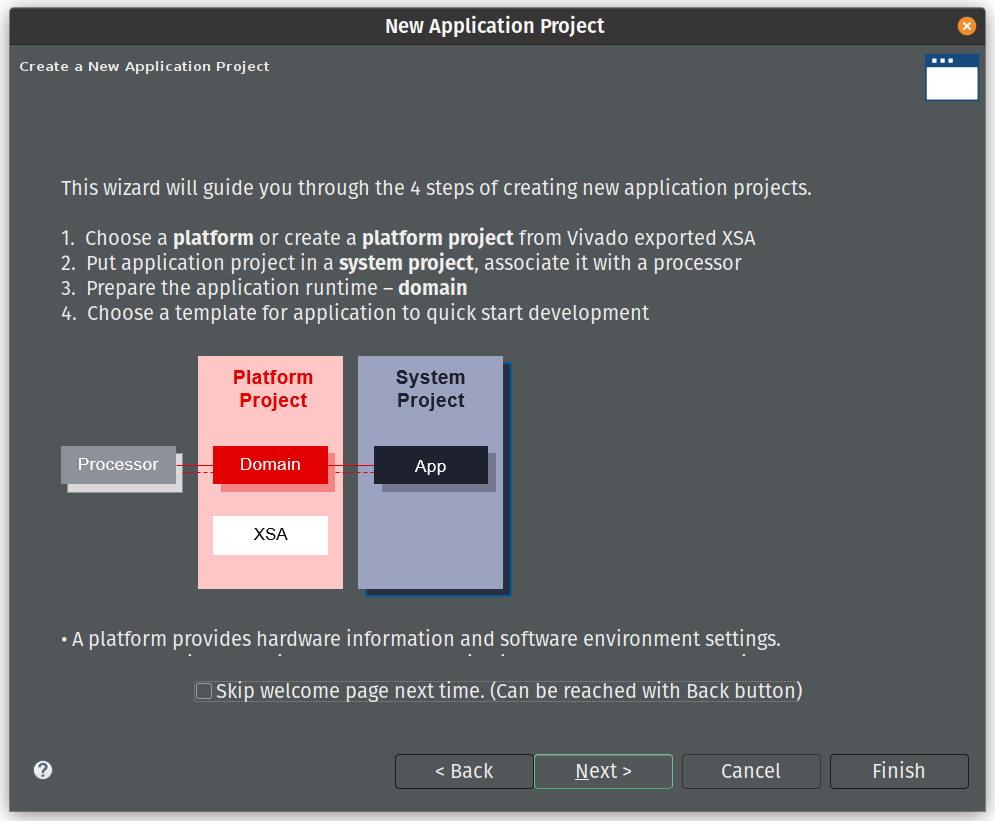
\includegraphics[width=.6\textwidth]{./img/vitis_new/project1.png}
\caption{\label{fig:org81f0e01}We are starting with creating a "New Application Project" You should be greeted with this wizard window. Next.}
\end{figure}

\begin{figure}[htbp]
\centering
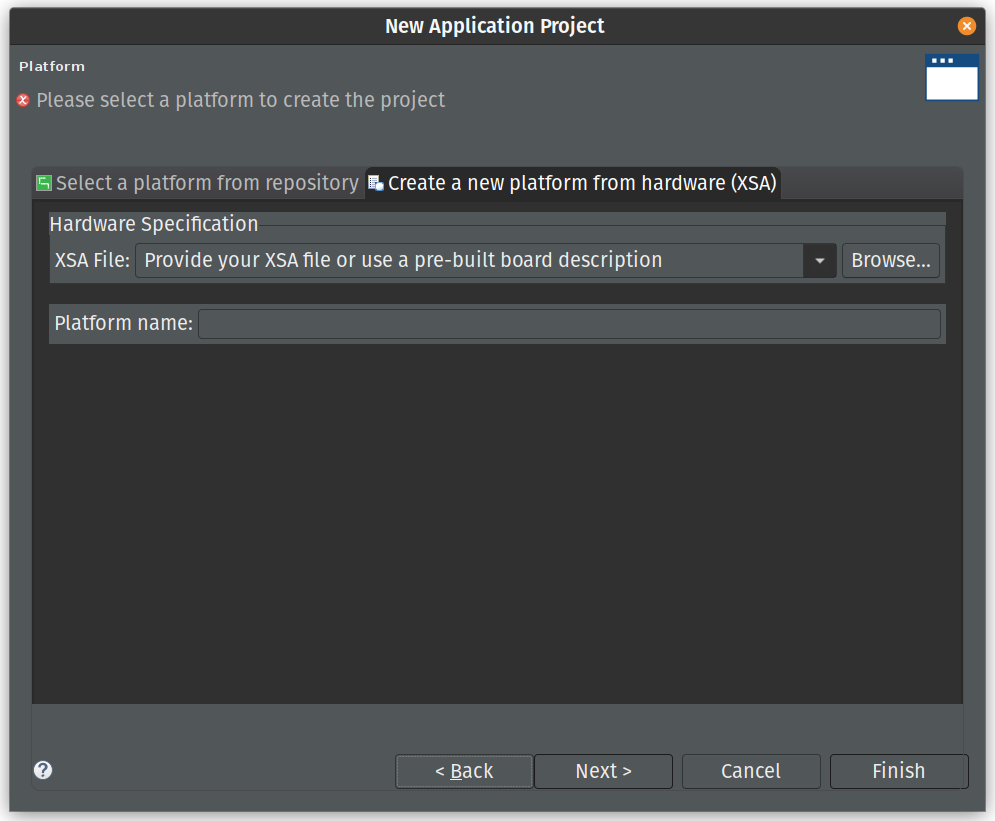
\includegraphics[width=.6\textwidth]{./img/vitis_new/project2.png}
\caption{\label{fig:org180be1b}For the platform, we need to get our build Kria configuration. In the "Create a new platform" tab, click the "Browse\ldots{}" button.}
\end{figure}

\begin{figure}[htbp]
\centering
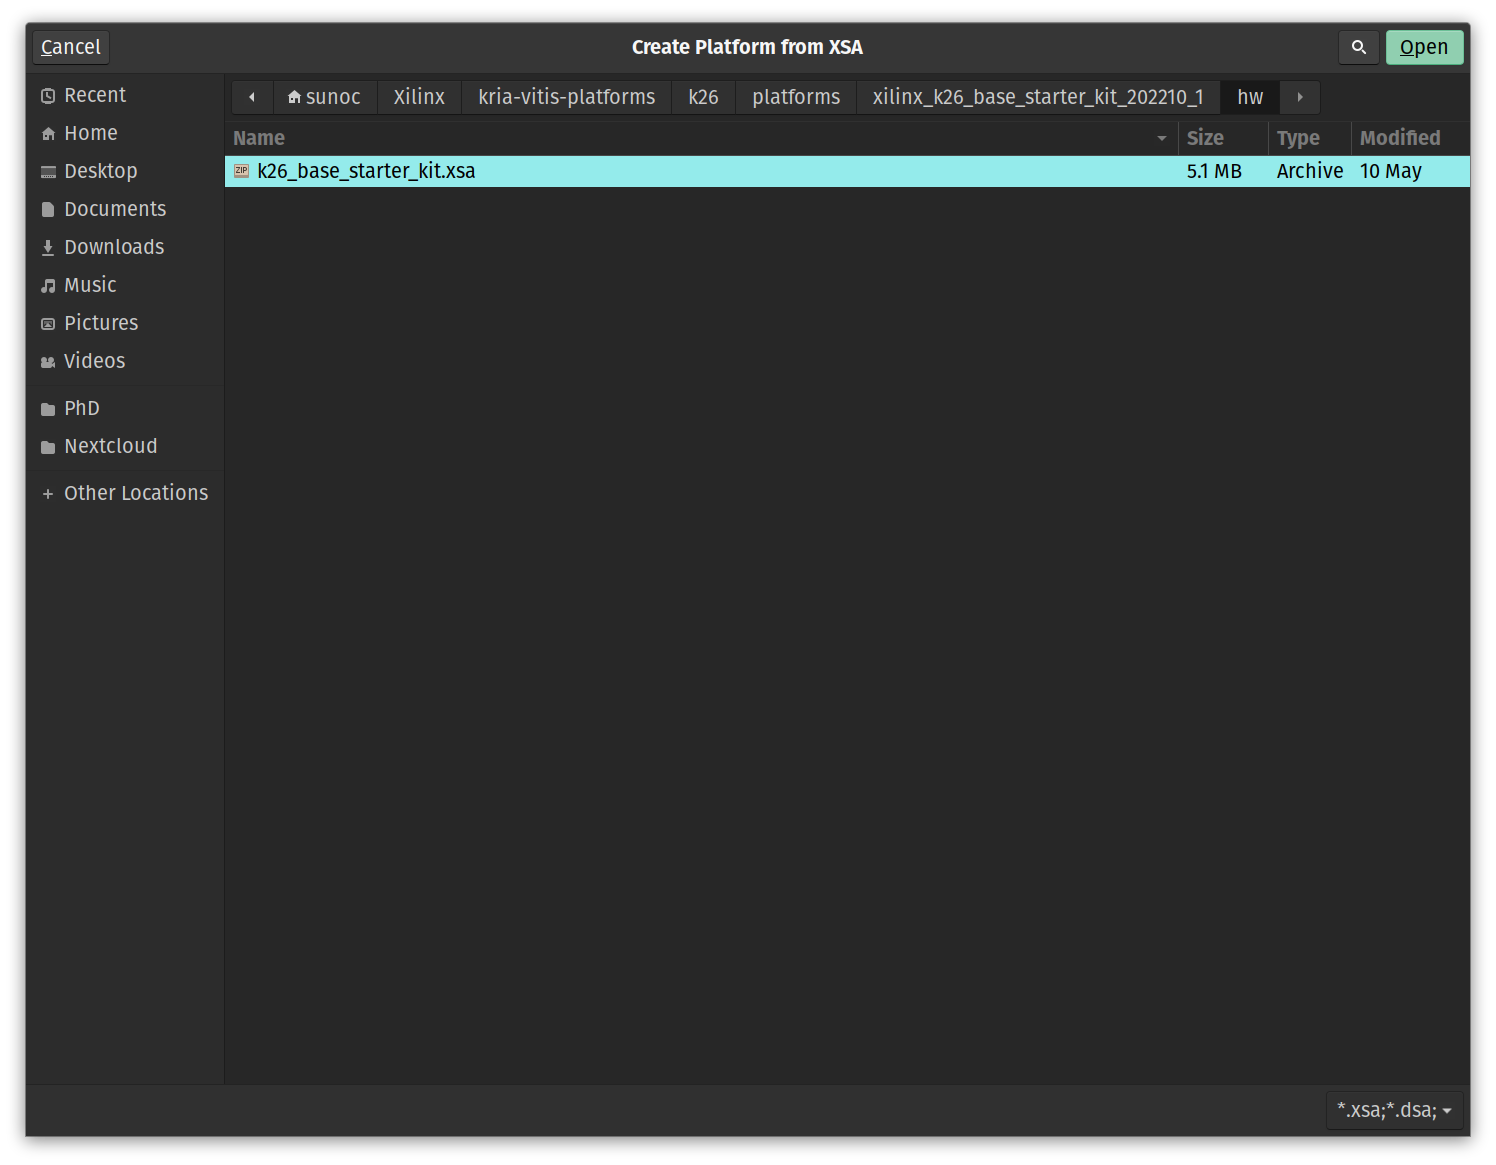
\includegraphics[width=.6\textwidth]{./img/vitis_new/project3.png}
\caption{\label{fig:org7edb00a}In the file explorer, we should navigate in the "k26" directory, where the configuration file was build. From here we are looking for a ".xsa" file, located in a "hw" directory, as visible.}
\end{figure}

\begin{figure}[htbp]
\centering
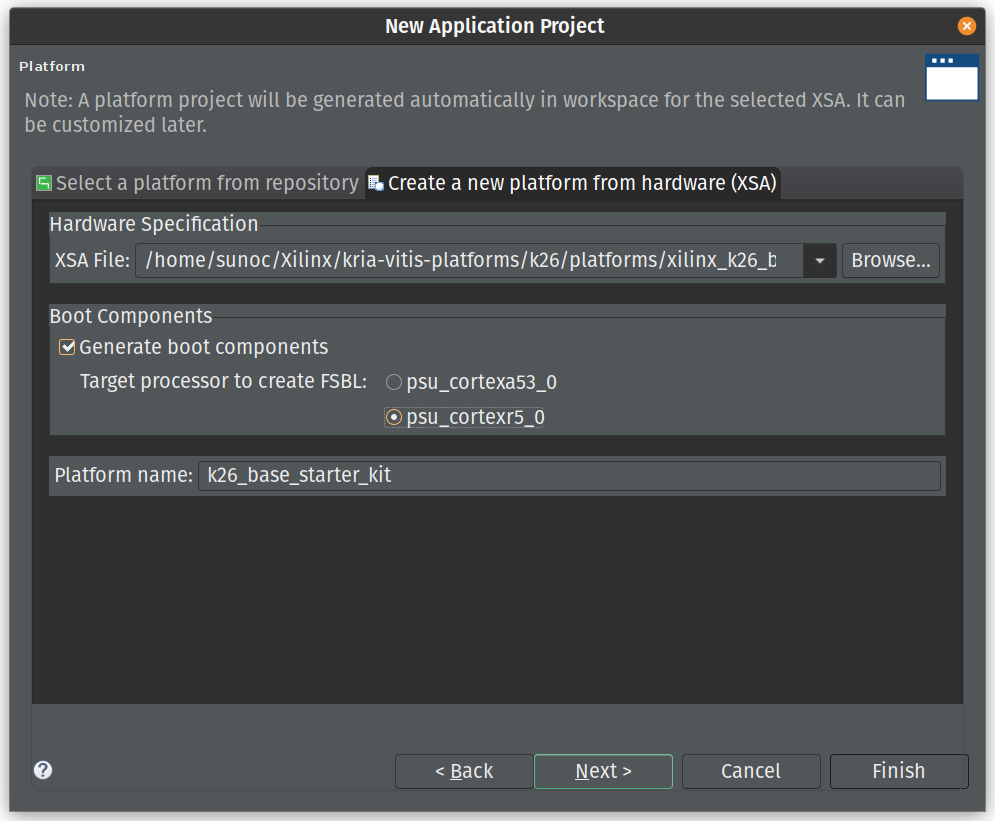
\includegraphics[width=.6\textwidth]{./img/vitis_new/project4.png}
\caption{\label{fig:org298e79e}With the configuration file loaded, we can now select a name for our platform, but most importantly, we have to select the "psu Cortex5 0" core as a target. The other, Cortex 53 is the APU running Linux.}
\end{figure}

\begin{figure}[htbp]
\centering
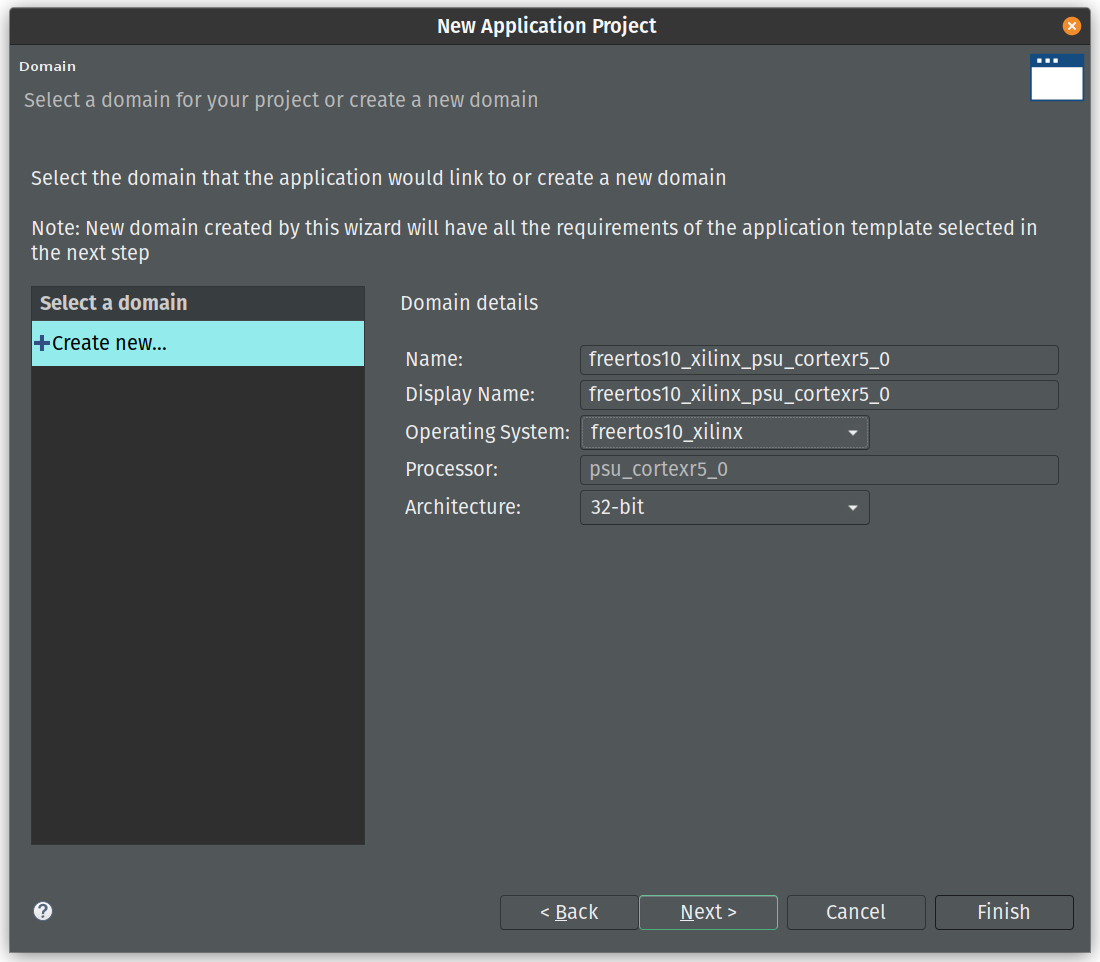
\includegraphics[width=.6\textwidth]{./img/vitis_new/project6.png}
\caption{\label{fig:orgb4386a3}Here, we want to select "freertos10 xilinx" as our Operating System. The rest can remain unchanged.}
\end{figure}

\begin{figure}[htbp]
\centering
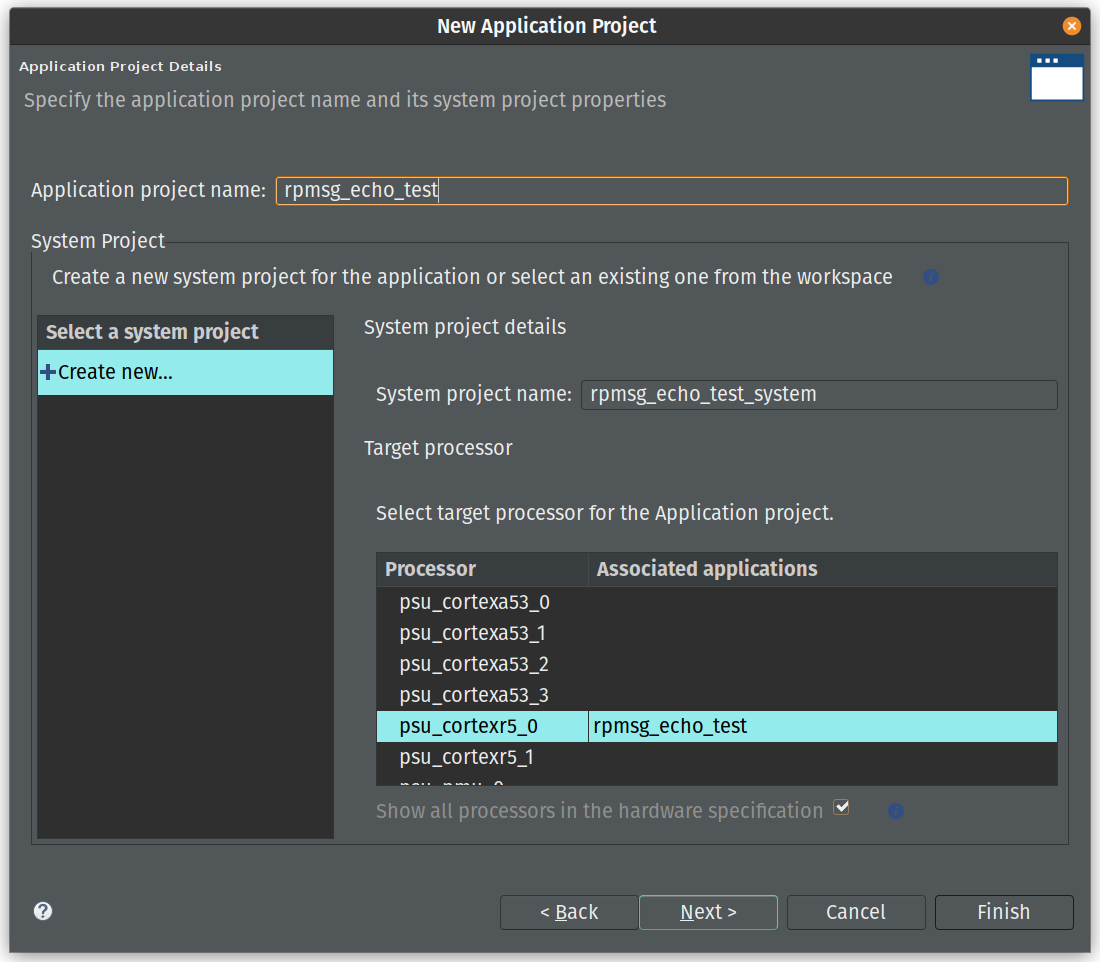
\includegraphics[width=.6\textwidth]{./img/vitis_new/project5.png}
\caption{\label{fig:org024196c}In this next window, we can give a name to our firmware project. It is also critical here to select the core we want to build for. Once again, we want to use the "psu cortex5 0".}
\end{figure}

\begin{figure}[htbp]
\centering
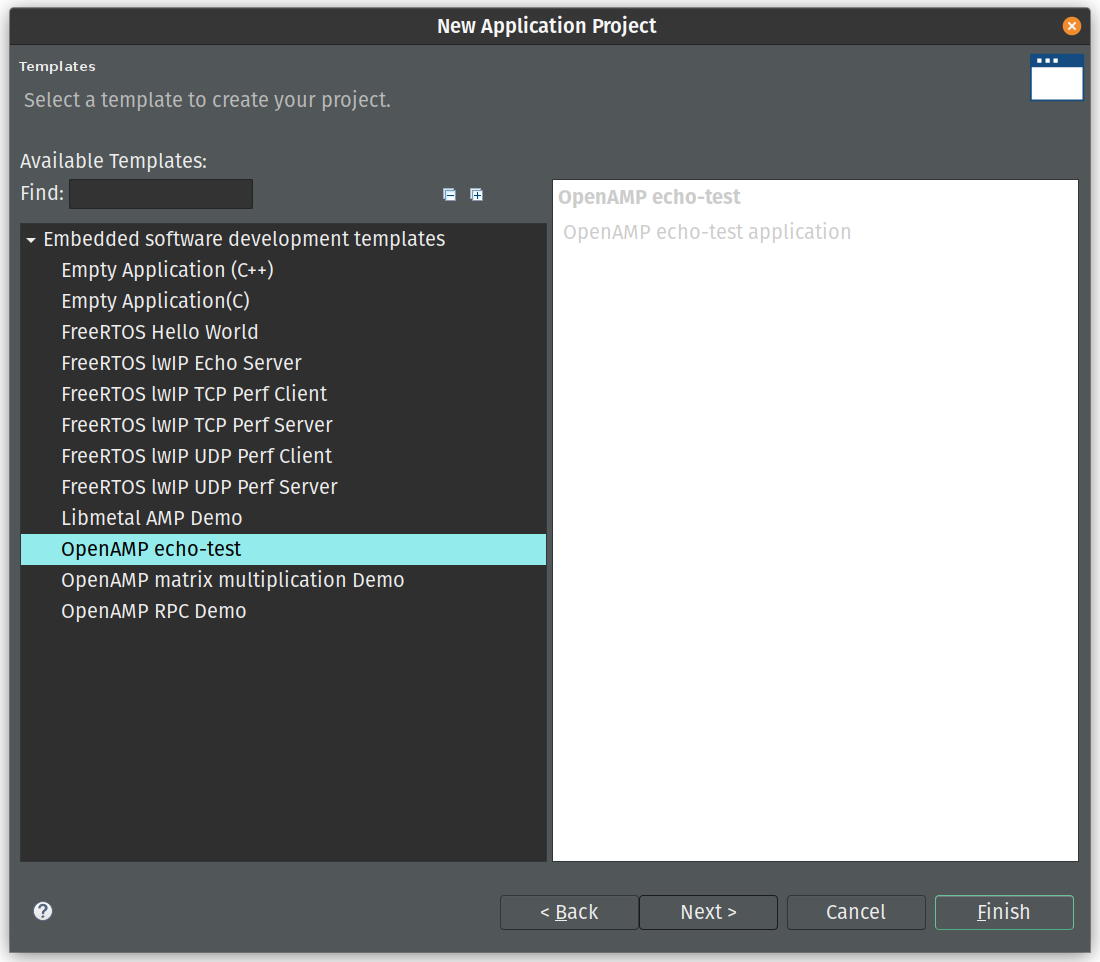
\includegraphics[width=.6\textwidth]{./img/vitis_new/project7.png}
\caption{\label{fig:org733a284}Finally, we can select the demonstration template we are going to use; here we go with "OpenAMP echo-test" since we want to have some simple try of the RPMsg system. Finish.}
\end{figure}

\pagebreak
In the Xilinx documentation, it is made mention of the addresses setting that should be checked in the \texttt{script.ld} file.
The values in the figure \ref{fig:orgfa0082c} below look different from what could be set in the DTO for the Linux side, but they appear to
work for the example we are running, including the new DTO patch without overlapping memory:


\begin{figure}[htbp]
\centering
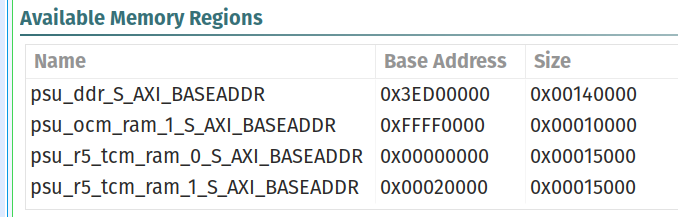
\includegraphics[width=.6\textwidth]{./img/vitis_new/project_mem.png}
\caption{\label{fig:orgfa0082c}lscript.ld memory configuration for the firmware memory setup. The same file is available as a whole in this repository's src directory.}
\end{figure}


Once your example project is built and you have a \texttt{.elf} file available, you can
jump directly in further sections to see how to deploy and use your firmware.

The section in between will present setup specifically needed for micro-ROS.

\section{Enabling the Stream Buffer system}
\label{sec:org551f874}
This is a subpart in the general configuration in the project related to some specific
functions for FreeRTOS threads messaging system, however, this point in particular
created so much pain I needed to include in early in this guide for not to forget about it
and keeping a clear track on how to enable this setting.

Indeed, two settings need to be enabled in order to be able to call
functions such as \texttt{xMessageBufferCreate}, useful when working with tasks
in FreeRTOS, as visible in the figure \ref{fig:orgb0442a3} below:

\begin{figure}[htbp]
\centering
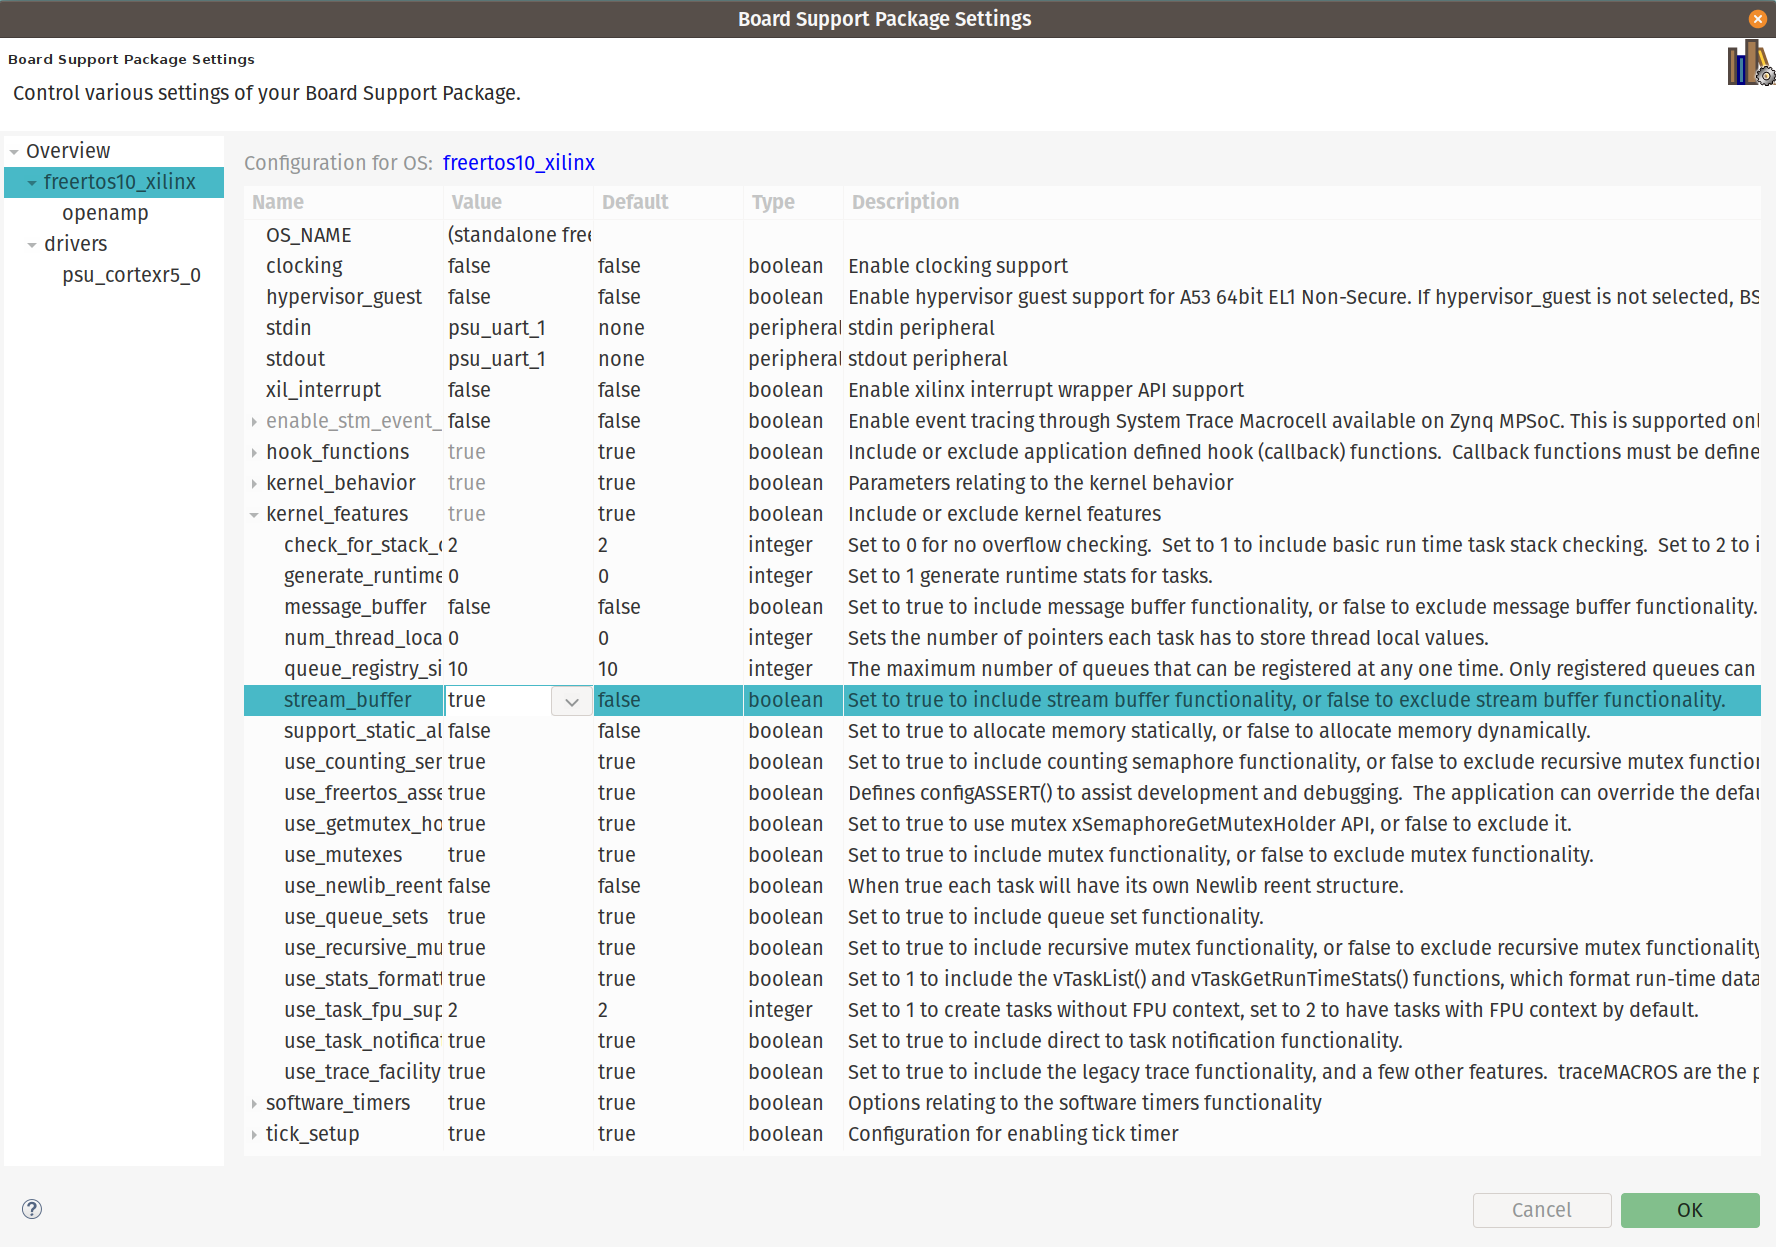
\includegraphics[width=.8\textwidth]{./img/streambuffer.png}
\caption{\label{fig:orgb0442a3}Enabling Stream Buffer in the Vitis IDE setting: this is a setting that can be found in the "platform.spr" element of your project (the platform, not the firmware project itself). From that file, you can access the settings with the button "Modify BSP Settings", and then as visible, in the tab \texttt{freertos10\_xilinx}, it is needed to toggle here the \texttt{stream\_buffer} setting in the \texttt{kernel\_features}, from the default "false" to "true".}
\end{figure}

\pagebreak
The second setting is useful in the case when a buffer callback function is used, such as\\[0pt]
\texttt{xMessageBufferCreateWithCallback}.
In that case, you must include \texttt{\#define configUSE\_SB\_COMPLETED\_CALLBACK 1} on the top of you header
file (in our project, this will happen in the \texttt{microros.h} header file),
before the \texttt{\#include "FreeRTOS.h"} in order to override the setting from this include.

\section{Including micro-ROS to the real-time firmware}
\label{sec:orgdb6991c}
Now we have a Vitis demonstration project available and the \texttt{libmicroros} static library
available, we can combine both by including this library into our Kria project.

On the host machine running the IDE, we can download the static library
and the include files from the Docker builder.
Here, we assume your Vitis IDE workspace sits in you home directory, at \texttt{\textasciitilde{}/workspace},
and that the Docker container is named \texttt{ros\_build}:
\begin{minted}[frame=single,framesep=2mm,baselinestretch=1.2,linenos,breaklines,fontsize=\footnotesize]{sh}
mkdir /home/$USER/workspace/microros_lib

docker cp ros_build:/microros_ws/firmware/build/\
       libmicroros.a /home/$USER/workspace/microros_lib/

docker cp ros_build:/microros_ws/firmware/build/include \
       /home/$USER/workspace/microros_lib/
\end{minted}

Many parameters are available to be set up in the IDE for the compilation tool-chain, but
the figures \ref{fig:org67627e0} and \ref{fig:orga935b54} below will show you a setup that worked to have the IDE
to recognize the include files and to be able to use them for compiling the firmware.

\begin{figure}[htbp]
\centering
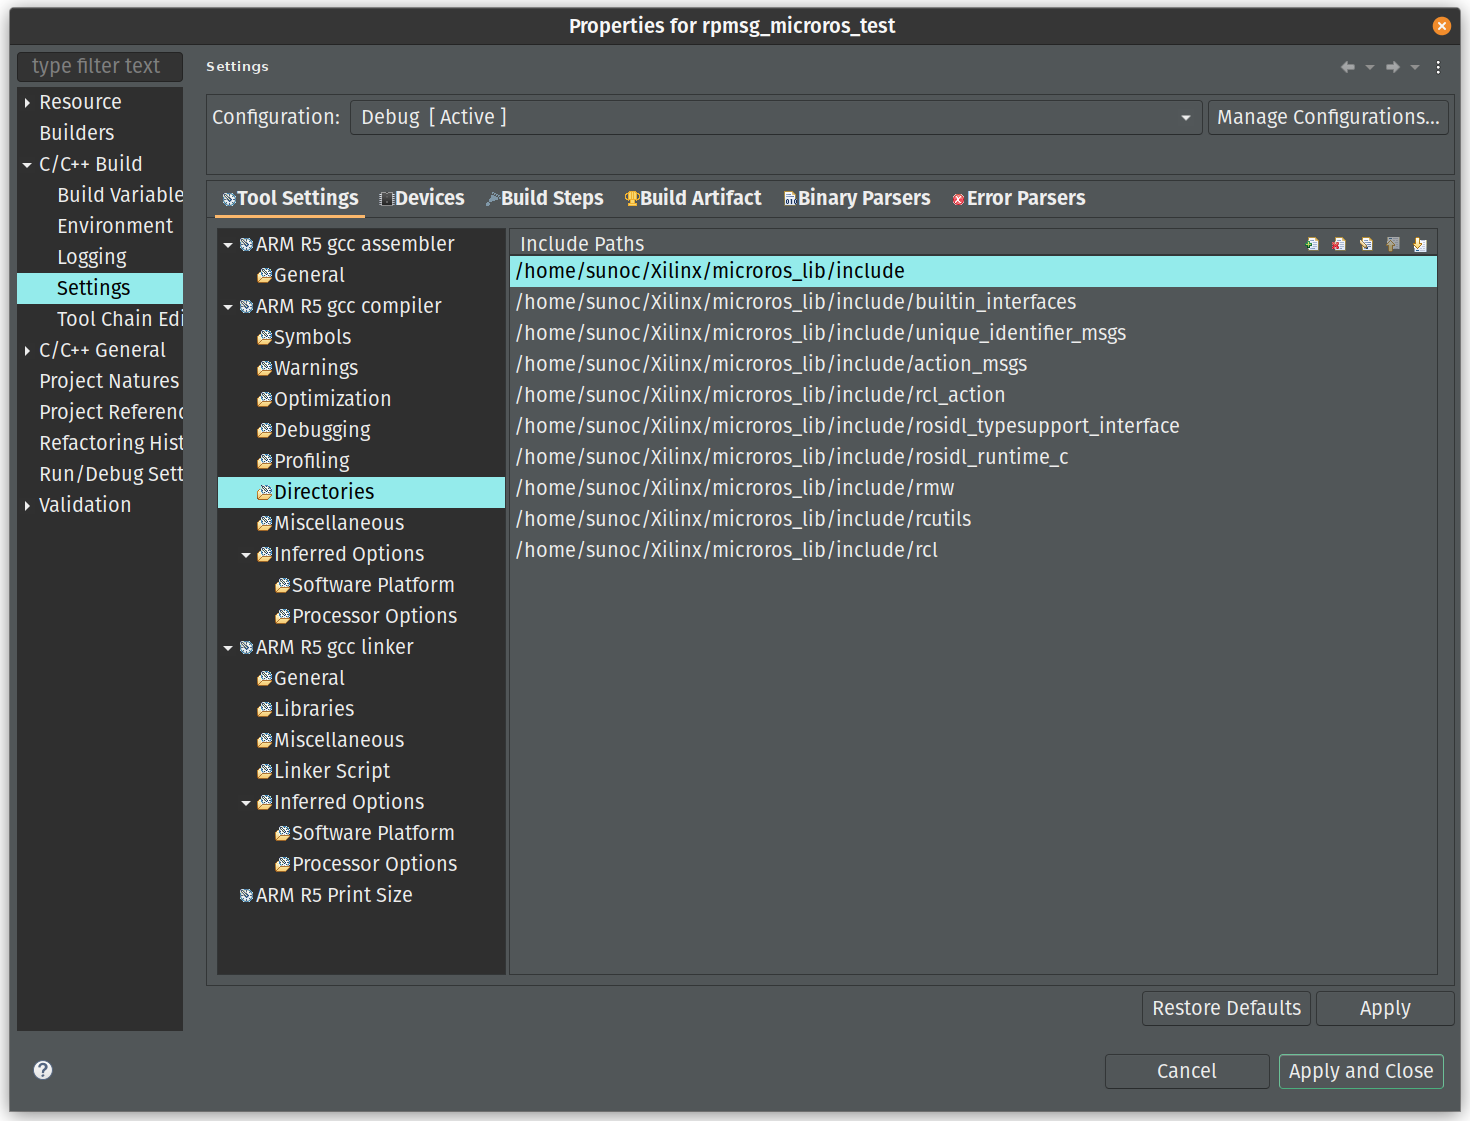
\includegraphics[width=.8\textwidth]{./img/vitis_new/include.png}
\caption{\label{fig:org67627e0}Firstly, in the "C/C++ Build" settings of your firmware project, under the "Settings" menu, you should find the gcc compiler "Directories". In here you should add the "include" directory of your library. Be careful however, if your include files are in a second layer of directory (as it is the case for libmicroros) you will need to include each sub-directory individually, as visible in this figure.}
\end{figure}

\begin{figure}[htbp]
\centering
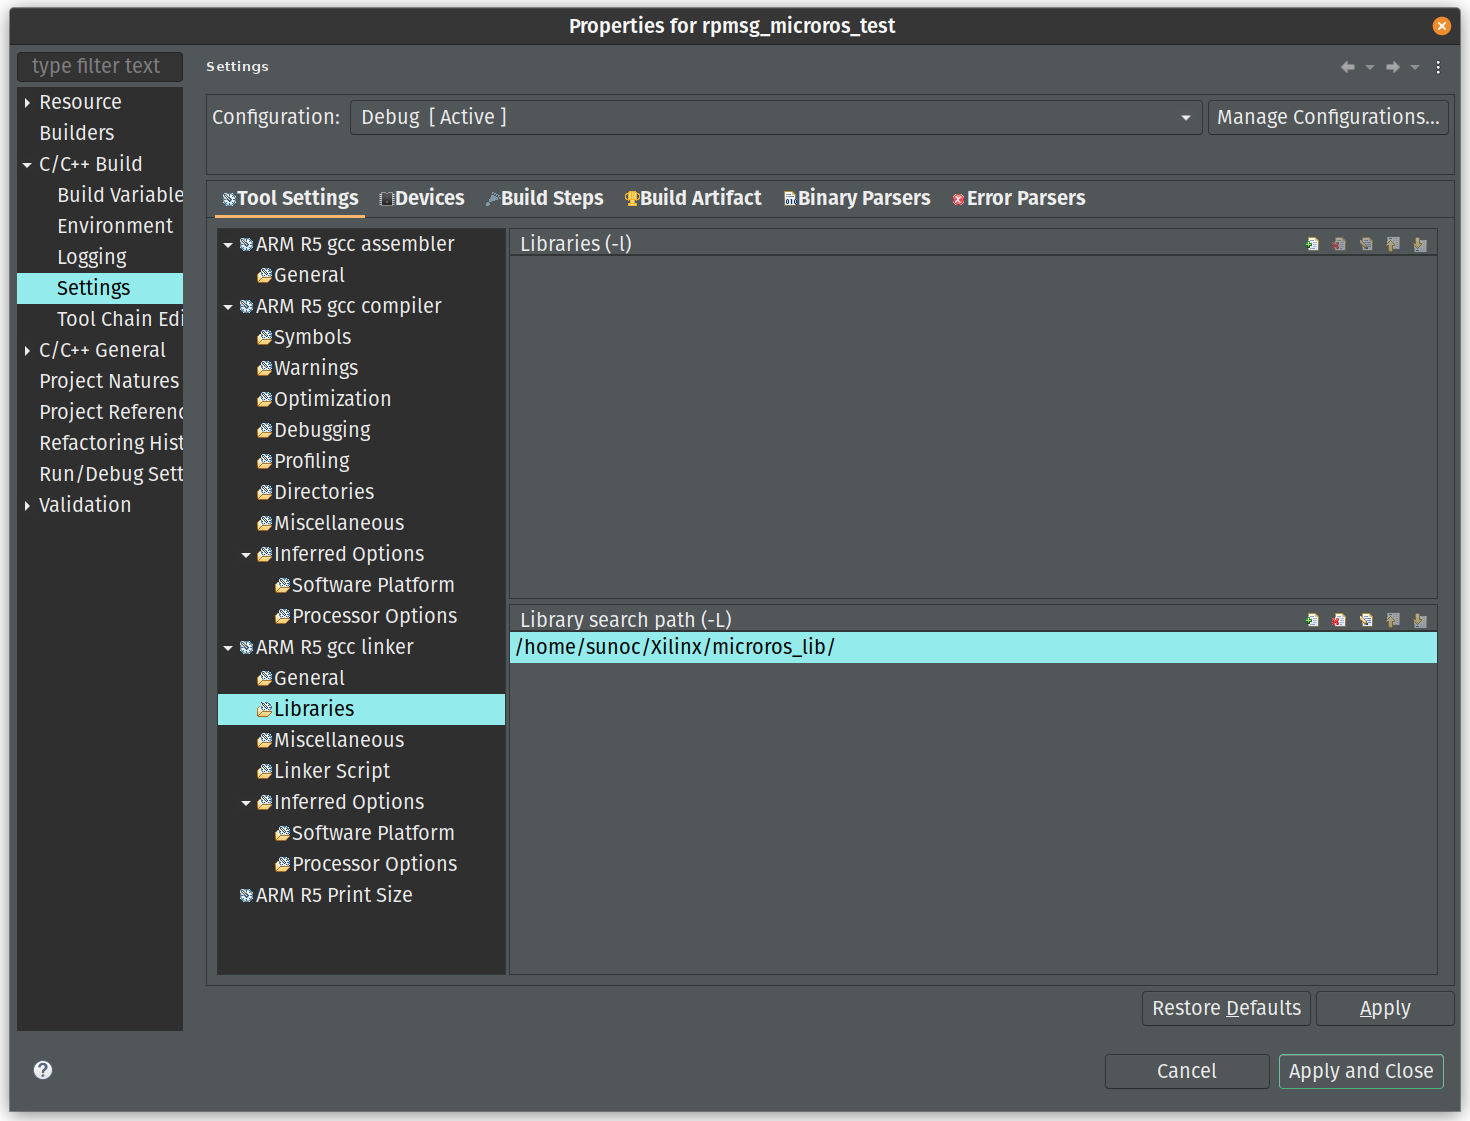
\includegraphics[width=.8\textwidth]{./img/vitis_new/include2.png}
\caption{\label{fig:orga935b54}Secondly, in the gcc linker "Libraries", you can add the top level directory of your library. In our case, it is the directory that contains both the "include" directory added earlier, and also the "libmicroros.a" file.}
\end{figure}

\pagebreak
With both of these setup in your project and as a minimal test to see if the setup was made correctly,
you should be able to include the following micro-ROS libraries into your project:
\begin{minted}[frame=single,framesep=2mm,baselinestretch=1.2,linenos,breaklines,fontsize=\footnotesize]{c}
#include <rcl/rcl.h>
#include <rcl/error_handling.h>
#include <rclc/rclc.h>
#include <rclc/executor.h>
\end{minted}

The details for the inclusions and the use-case of the library will depend on the implementation
of the firmware itself.
\end{document}
